\chapter{Résultats}

Les résultats suivants ont été obtenus à l'aide du module \pyth{stats.py}.\\
La figure donne : 
\begin{itemize}
	\item L'histogramme de répartition des scores \\
	(on rappelle que : 1 ligne  $\rightarrow 40$, 2 lignes$\rightarrow 100$, 3 lignes $\rightarrow 300$ et 4 lignes $\rightarrow 1200$)
	\item La moyenne et l'écart-type
	\item Le diagramme en boîte des résultats (minimum, $Q_1$, médiane, $Q_3$ et maximum)
\end{itemize}

Sauf indication contraire, on ne limite pas le nombre de blocs joués (ce qui fait que les tests ont été particulièrement longs à effectuer) et on teste sur 100 parties.

\section{Agents par filtrage}

Agent par filtrage en filtrant, dans l'ordre, les trous, la somme des hauteurs, le bumpiness et le nombre de lignes :

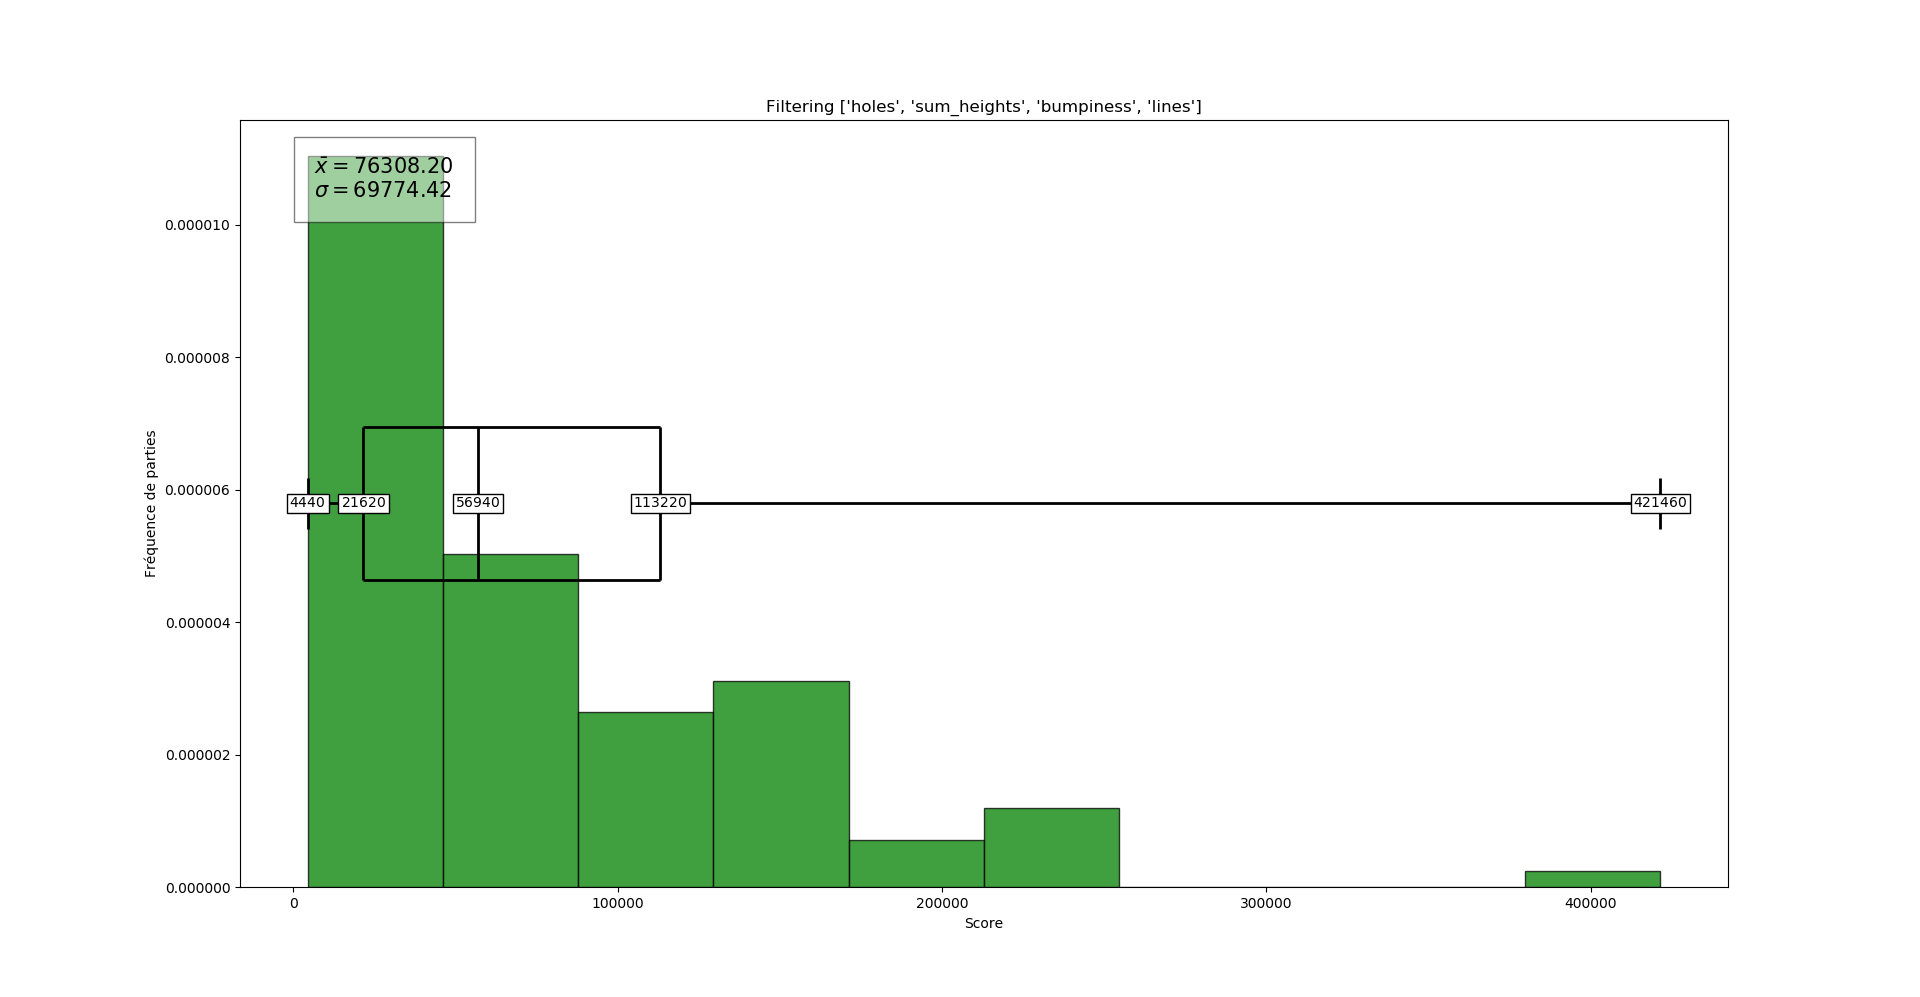
\includegraphics[scale=0.35]{media/results/Stats_Filtering_H_SH_B_L_n=100.png}

\newpage

\section{Algorithmes génétiques}

Voici différents résultats d'optimisation par algorithmes génétiques en variant les différents paramètres. \\
Afin d'obtenir des résultats comparables et de ne pas avoir de temps de calculs trop longs, nous avons fixé les paramètres suivants dans toutes les optimisations :
\begin{itemize}
	\item Taille de la population : 100
	\item Nombre de générations : 20
	\item Nombre maximum de blocs joués : 500
	\item Nombre de parties pour l'évaluation : 5
\end{itemize} 

\newpage

\subsection{Exemple 1}
Paramètres :
\begin{itemize}
	\item \pyth{vector\_encoding : float}
	\item \pyth{parents\_selection\_method : tournament}
	\item \pyth{old\_generation\_policy : best}
	\item \pyth{evaluation\_criteria : lines}
	\item \pyth{proba\_mutation = 0.05}
	\item \pyth{mutation\_rate = 0.20}
	\item \pyth{percentage\_for\_tournament = 0.10}
	\item \pyth{percentage\_new\_offspring = 0.30}
\end{itemize} 

L'optimisation a duré à peu près 5 heures. Voici l'évolution de la population :

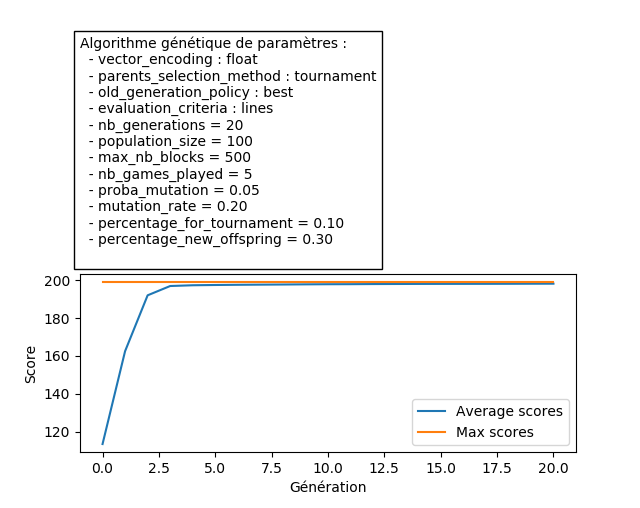
\includegraphics[scale=0.95]{media/results/AG01.png}

On voit que si la population a une tendance moyenne à fortement augmenter, le meilleur individu stagne. En fait ça a été le même durant toutes les générations.\\
En effet, l'évaluation des agents se faisant sur le nombre de lignes, il semble qu'un maximum de 200 lignes ne puisse pas vraiment être dépassé. Toutes les optimisations avec une évaluation sur les lignes ont donné à peu près le même type de résultat. C'est pourquoi dans les exemples suivants nous prendrons une évaluation sur les scores.

\medskip

Le meilleur individu a pour coefficients : \pyth{[0.7389, 0.5367, 0.3951, 0.0997]}.
\newpage

Regardons ses statistiques sur 100 parties :

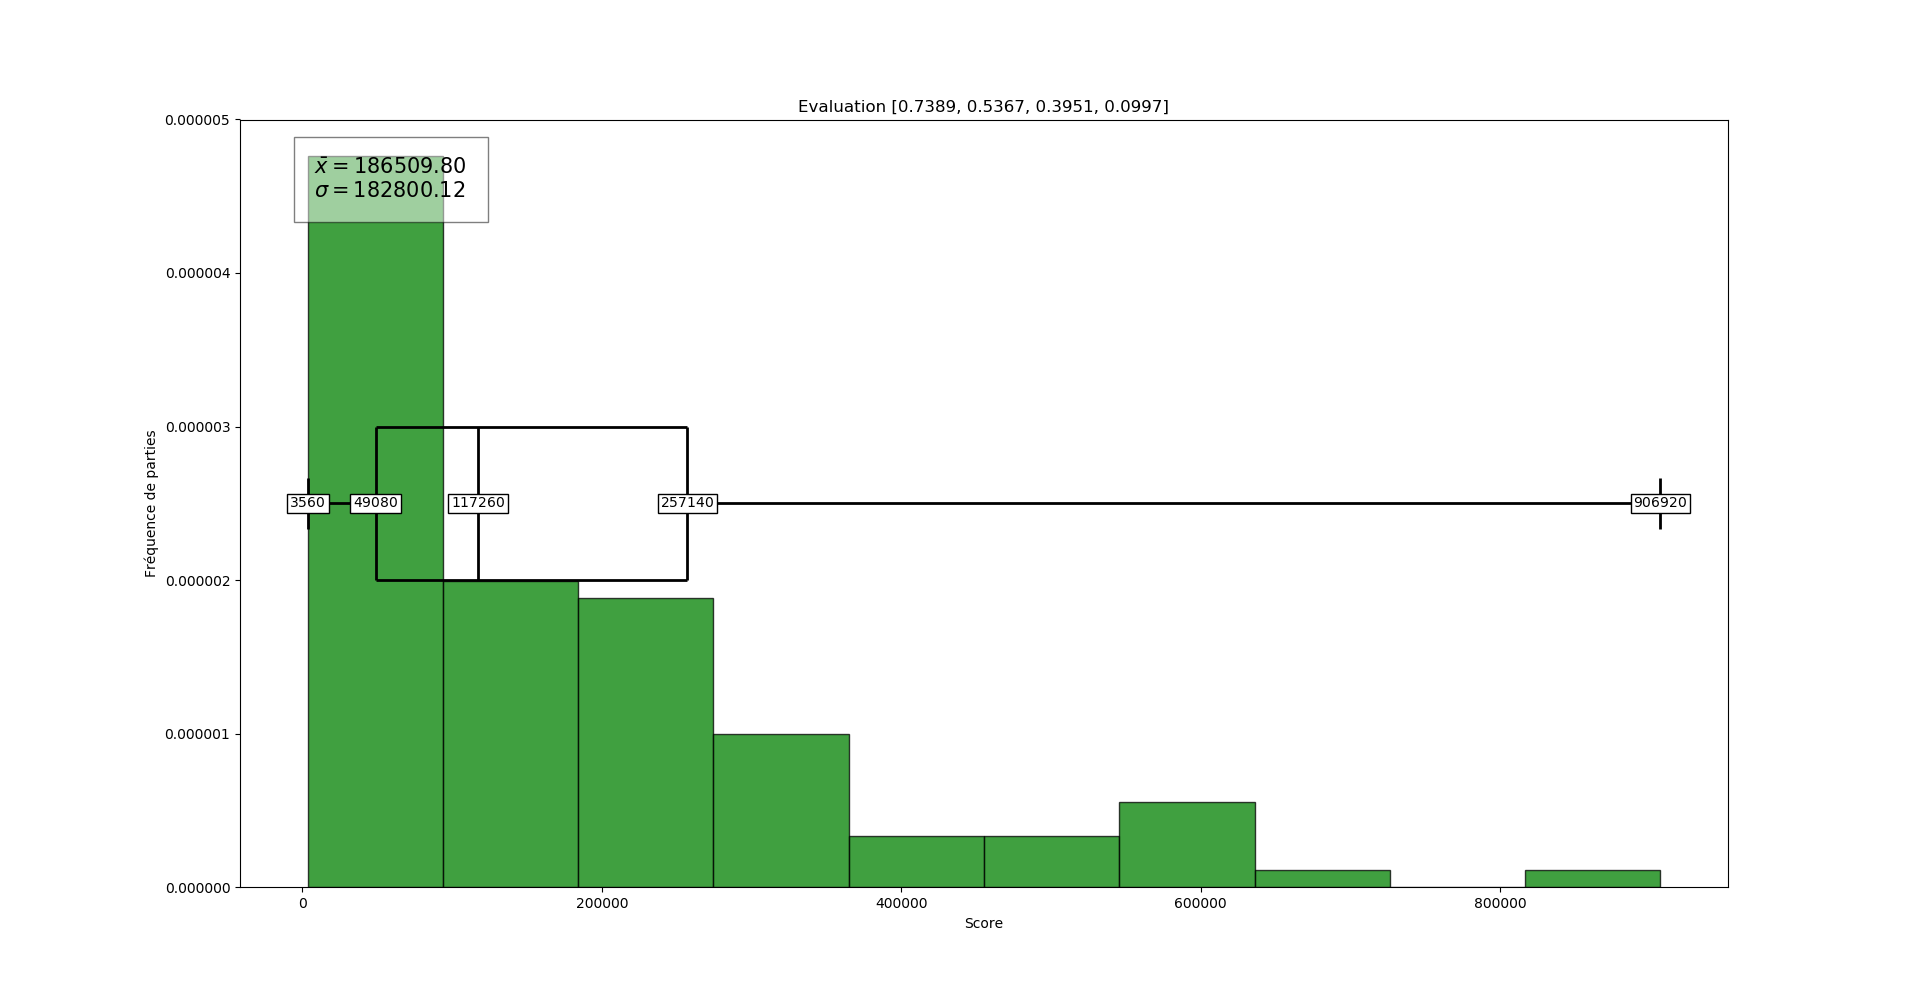
\includegraphics[scale=0.35]{media/results/Stats_Eval_0,7389_0,5367_0,3951_0,0997.png}

\newpage

\subsection{Exemple 2}

Paramètres :
\begin{itemize}
	\item \pyth{vector\_encoding : float}
	\item \pyth{parents\_selection\_method : tournament}
	\item \pyth{old\_generation\_policy : best}
	\item \pyth{evaluation\_criteria : scores}
	\item \pyth{proba\_mutation = 0.05}
	\item \pyth{mutation\_rate = 0.20}
	\item \pyth{percentage\_for\_tournament = 0.10}
	\item \pyth{percentage\_new\_offspring = 0.30}
\end{itemize} 

L'optimisation a duré à peu près 3 heures. Voici l'évolution de la population :

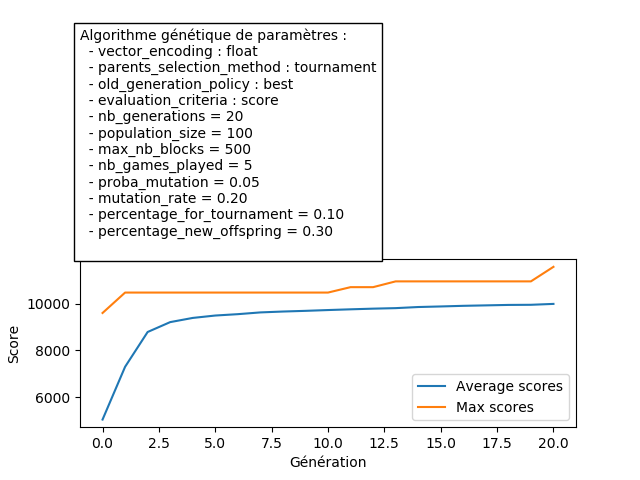
\includegraphics[scale=0.95]{media/results/AG11.png}

Ici la population a une tendance moyenne à fortement augmenter,  et le meilleur individu augmente également. 

\medskip

Le meilleur individu a pour coefficients : \pyth{[0.5037, 0.7762, 0.3666, 0.0967]}.
\newpage

Regardons ses statistiques sur 100 parties :

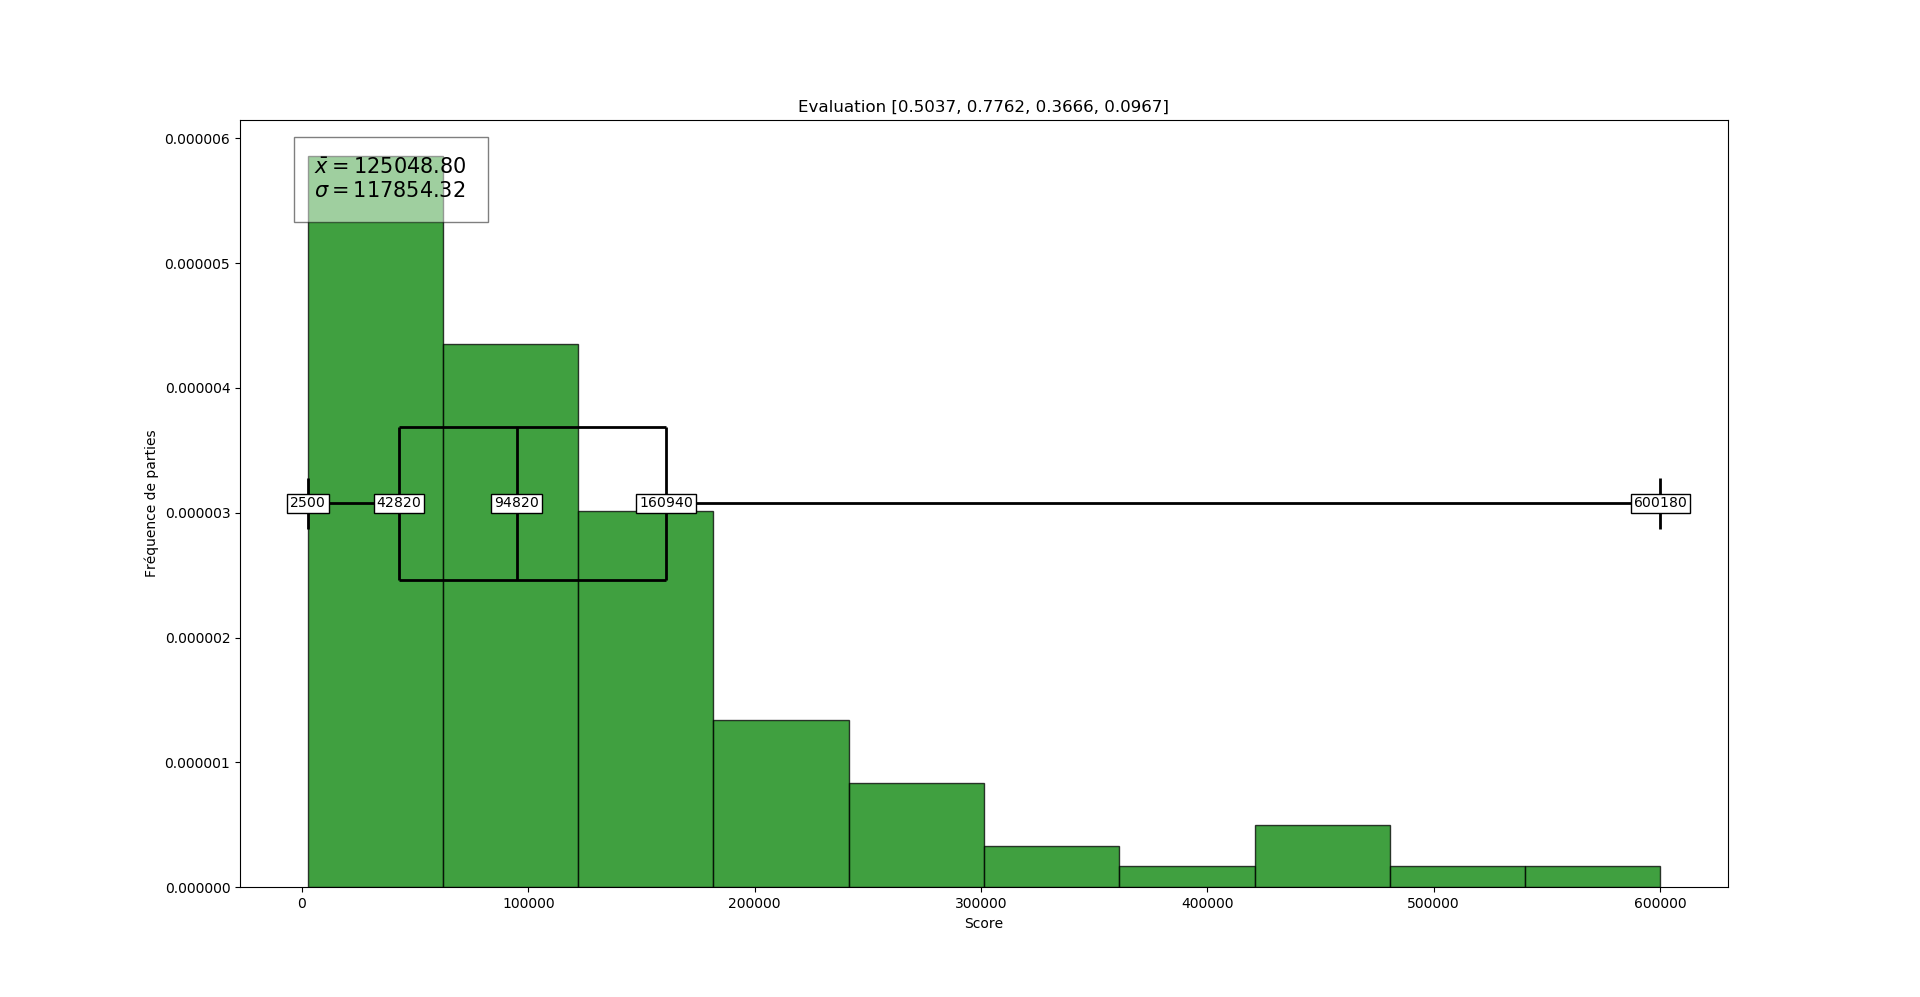
\includegraphics[scale=0.35]{media/results/Stats_Eval_0,5037_0,7762_0,3666_0,0967.png}

\newpage

\subsection{Exemple 3}

Dans cet exemple nous avons simplement changé l'encodage des individus :

Paramètres :
\begin{itemize}
	\item \pyth{vector\_encoding : bin}
	\item \pyth{parents\_selection\_method : tournament}
	\item \pyth{old\_generation\_policy : best}
	\item \pyth{evaluation\_criteria : scores}
	\item \pyth{proba\_mutation = 0.05}
	\item \pyth{percentage\_for\_tournament = 0.10}
	\item \pyth{percentage\_new\_offspring = 0.30}
\end{itemize} 

L'optimisation a duré à peu près 3 heures. Voici l'évolution de la population :

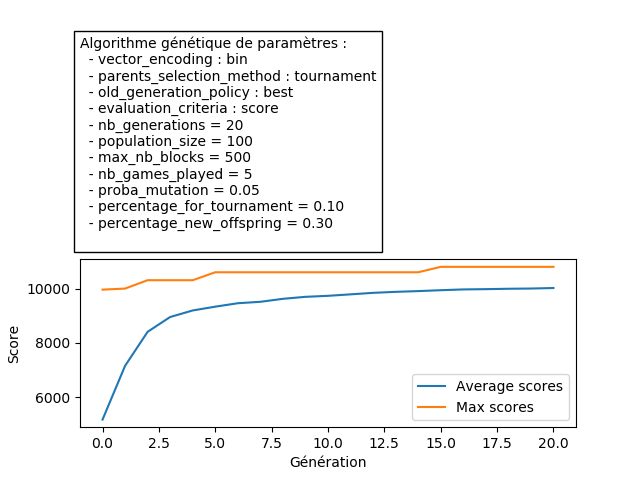
\includegraphics[scale=0.95]{media/results/AG10.png}

On obtient le même profil que précédemment en changeant l'encodage.

\medskip

Le meilleur individu a pour coefficients : \pyth{[0.2173, 0.4716, 0.9472, 0.1798]}.
\newpage

Regardons ses statistiques sur 100 parties :

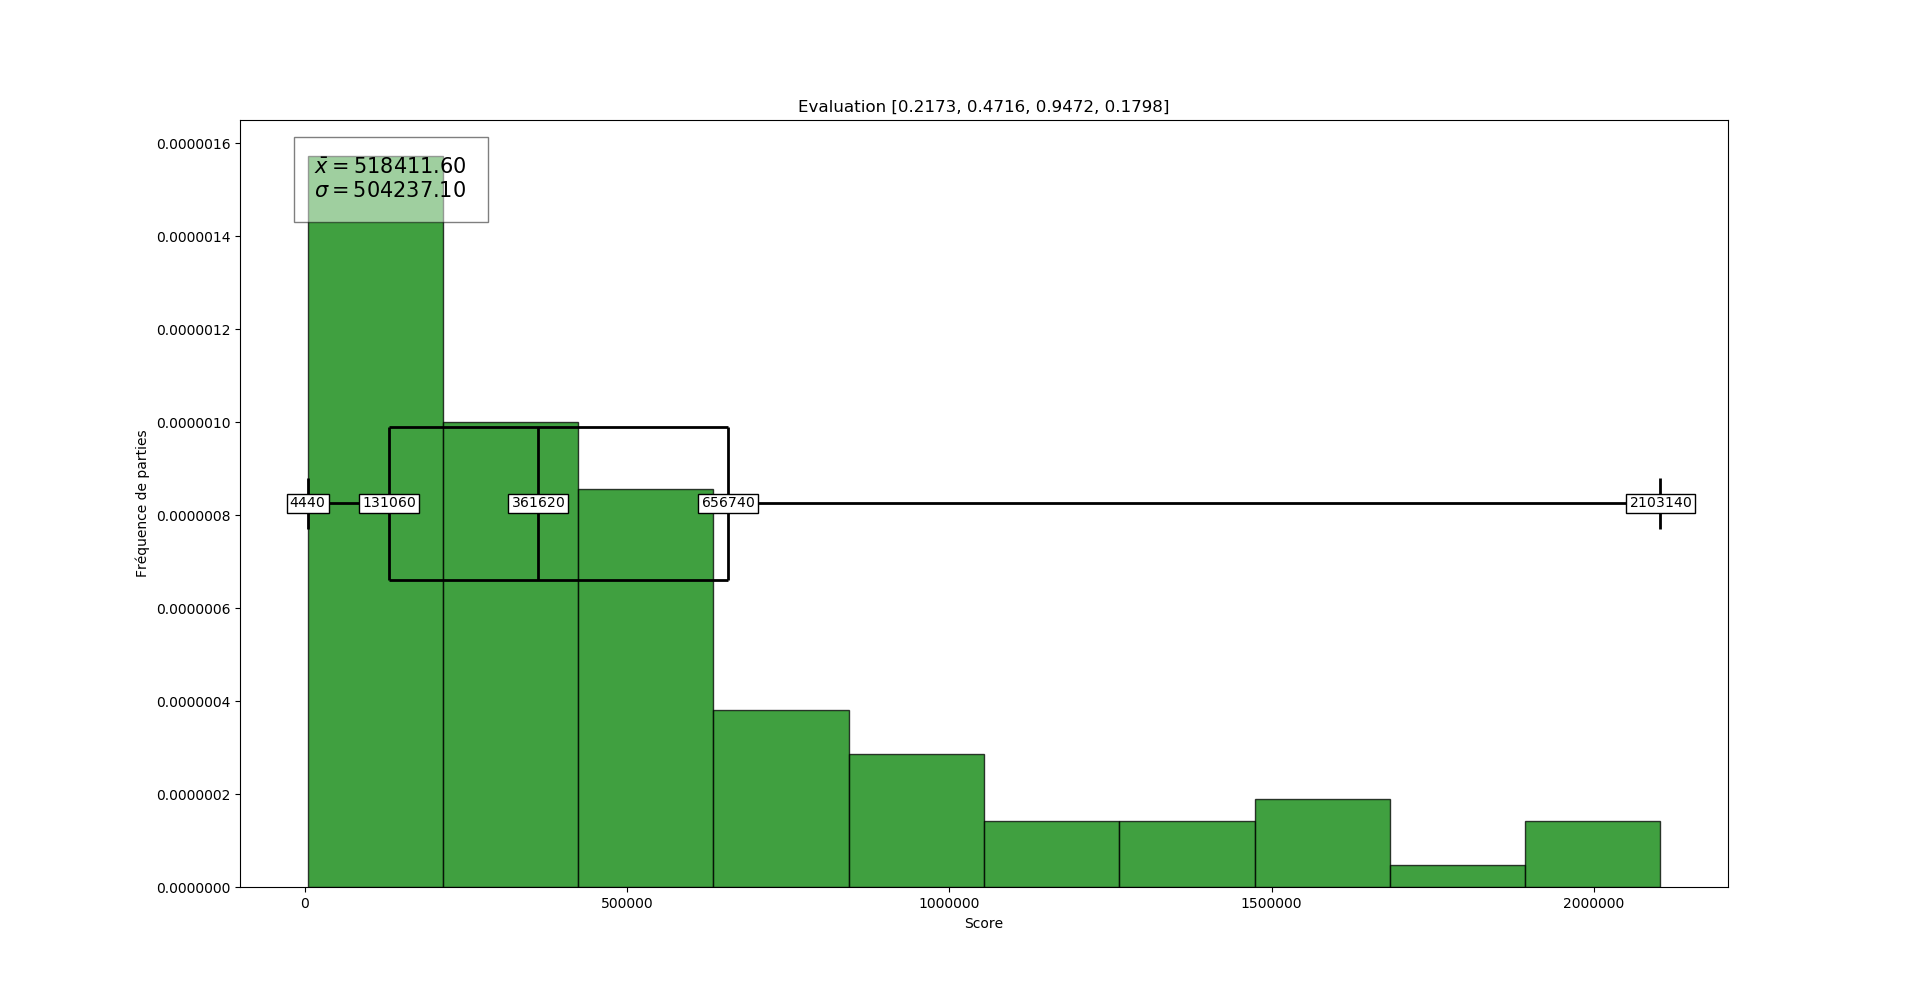
\includegraphics[scale=0.35]{media/results/Stats_Eval_0,2173_0,4716_0,9472_0,1798.png}

\newpage

\subsection{Exemple 4}

Dans cet exemple nous avons changé le mode de conservation des anciens individus :

Paramètres :
\begin{itemize}
	\item \pyth{vector\_encoding : bin}
	\item \pyth{parents\_selection\_method : tournament}
	\item \pyth{old\_generation\_policy : elitism}
	\item \pyth{evaluation\_criteria : scores}
	\item \pyth{proba\_mutation = 0.05}
	\item \pyth{percentage\_for\_tournament = 0.10}
	\item \pyth{elitism\_percentage = 0.10}
\end{itemize} 

L'optimisation a duré à peu près 12 heures ce qui est considérablement plus long. Voici l'évolution de la population :

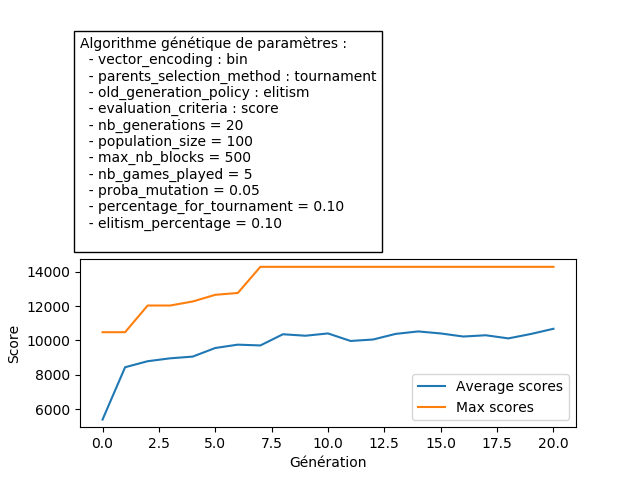
\includegraphics[scale=0.95]{media/results/AG12.png}

On n'a plus ce phénomène de population moyenne qui se stabilise sur le maximum. En revanche, on constate une nette évolution du meilleur individu.

\medskip

Le meilleur individu a pour coefficients : \pyth{[0.0.016, 0.007, 0.5937, 0.0198]}.
\newpage

Regardons ses statistiques sur 100 parties :

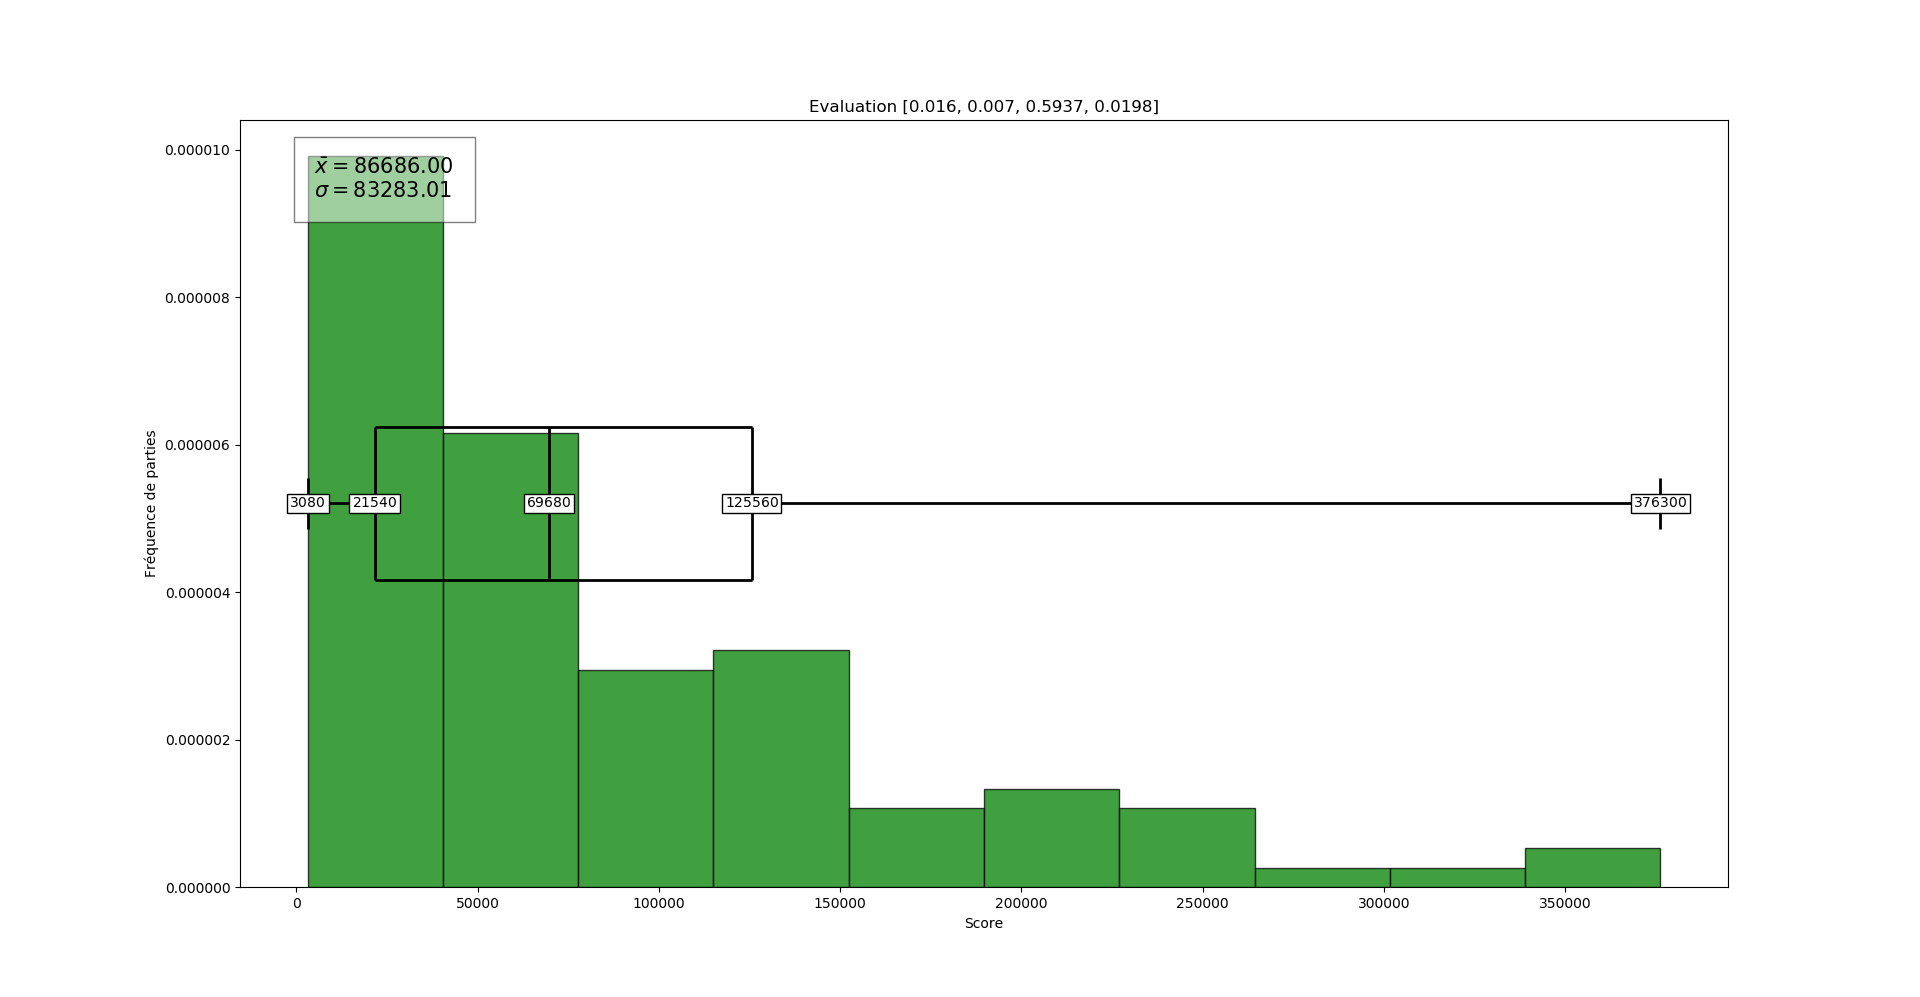
\includegraphics[scale=0.35]{media/results/Stats_Eval_0,016_0,007_0,5937_0,0198.png}

\newpage

\subsection{Exemple 5}

Ici, nous avons changé le mode de sélection des individus :

Paramètres :
\begin{itemize}
	\item \pyth{vector\_encoding : bin}
	\item \pyth{parents\_selection\_method : wheel}
	\item \pyth{old\_generation\_policy : elitism}
	\item \pyth{evaluation\_criteria : scores}
	\item \pyth{proba\_mutation = 0.05}
	\item \pyth{percentage\_for\_tournament = 0.10}
	\item \pyth{elitism\_percentage = 0.10}
\end{itemize} 

L'optimisation a encore duré à peu près 12 heures. Voici l'évolution de la population :

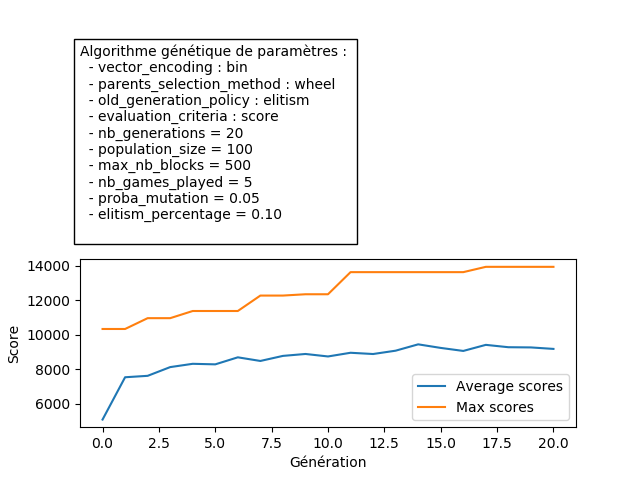
\includegraphics[scale=0.95]{media/results/AG14.png}

On observe le même profil que précédemment.

\medskip

Le meilleur individu a pour coefficients : \pyth{[0.27, 0.0105, 0.839, 0.0472]}.
\newpage

Regardons ses statistiques sur 100 parties :

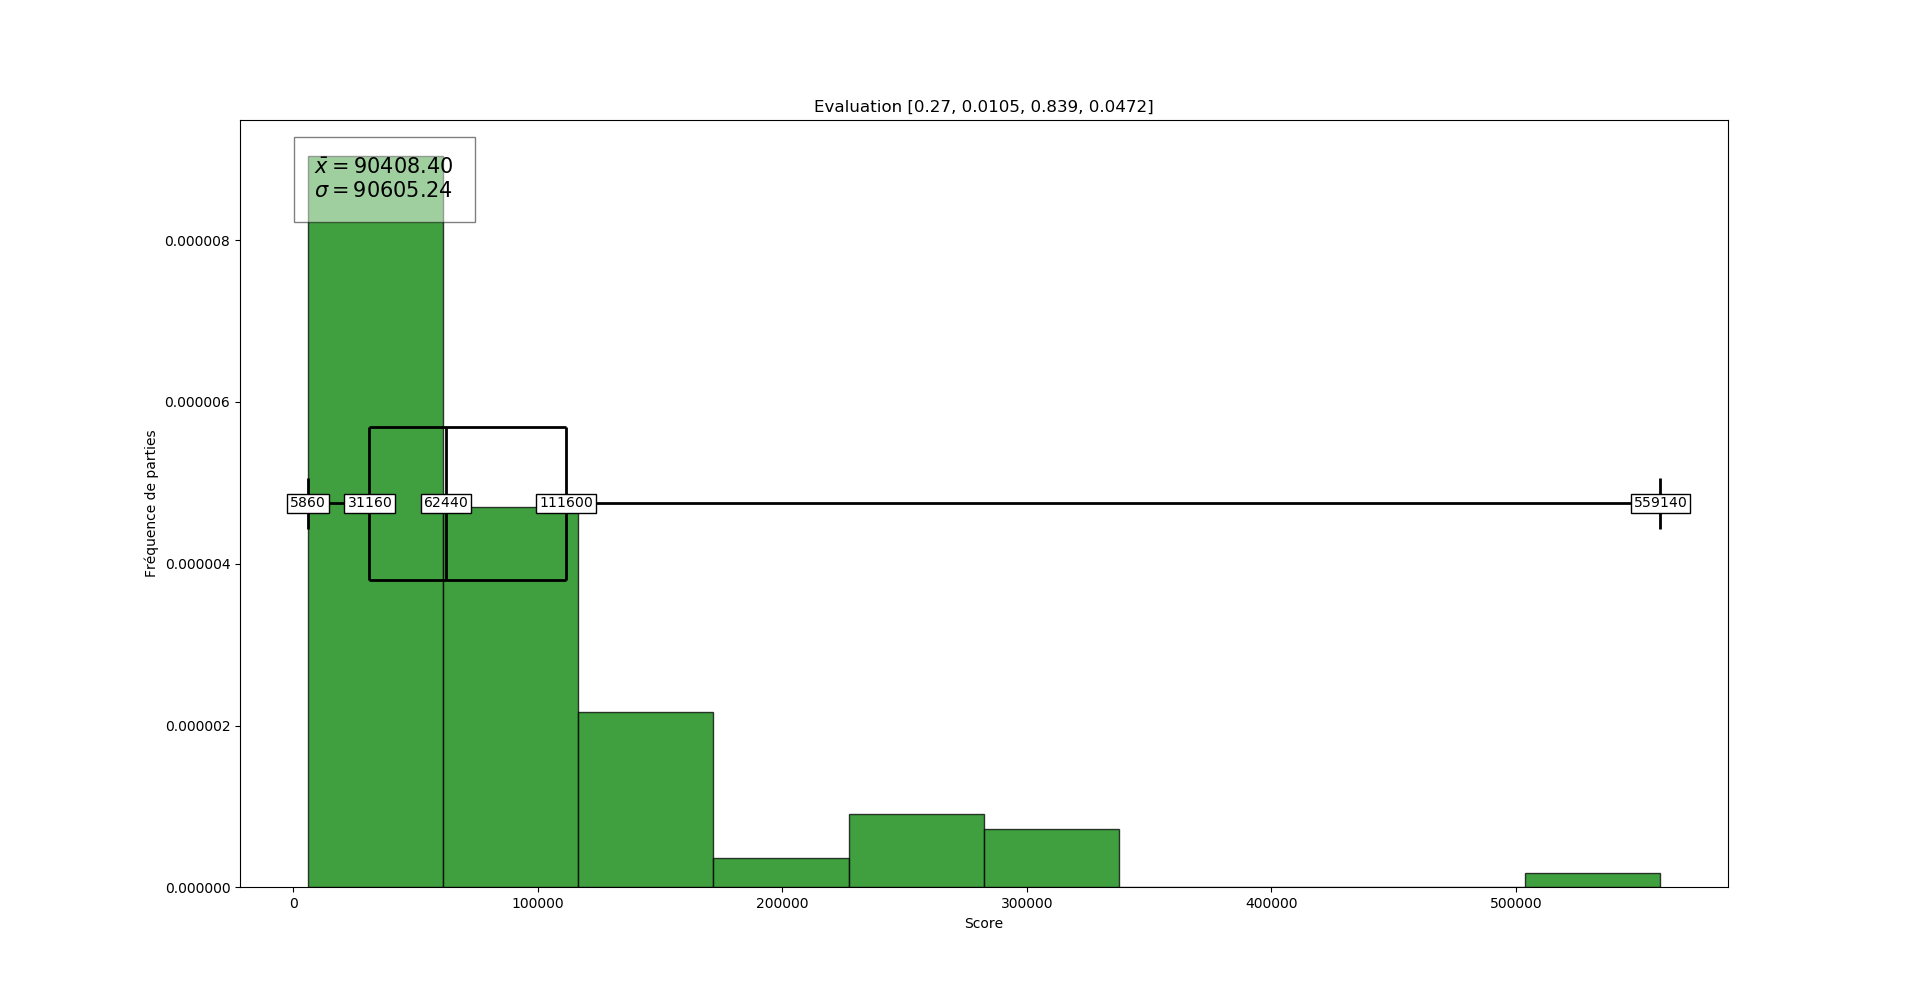
\includegraphics[scale=0.35]{media/results/Stats_Eval_0,27_0,0105_0,839_0,0472.png}

\newpage

\subsection{Exemple 5}

Enfin nous avons ajouté de la mutation :

Paramètres :
\begin{itemize}
	\item \pyth{vector\_encoding : bin}
	\item \pyth{parents\_selection\_method : wheel}
	\item \pyth{old\_generation\_policy : elitism}
	\item \pyth{evaluation\_criteria : scores}
	\item \pyth{proba\_mutation = 0.1}
	\item \pyth{percentage\_for\_tournament = 0.10}
	\item \pyth{elitism\_percentage = 0.10}
\end{itemize} 

L'optimisation a encore duré à peu près 12 heures. Voici l'évolution de la population :

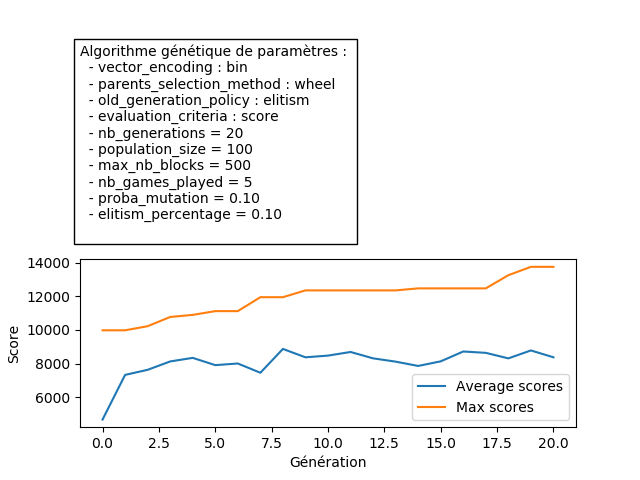
\includegraphics[scale=0.95]{media/results/AG13.png}

Le meilleur individu augmente sensiblement. En revanche, la population moyenne semble dégénérer.

\medskip

Le meilleur individu a pour coefficients : \pyth{[0.1407, 0.0039, 0.7186, 0.0455]}.
\newpage

Regardons ses statistiques sur 100 parties :

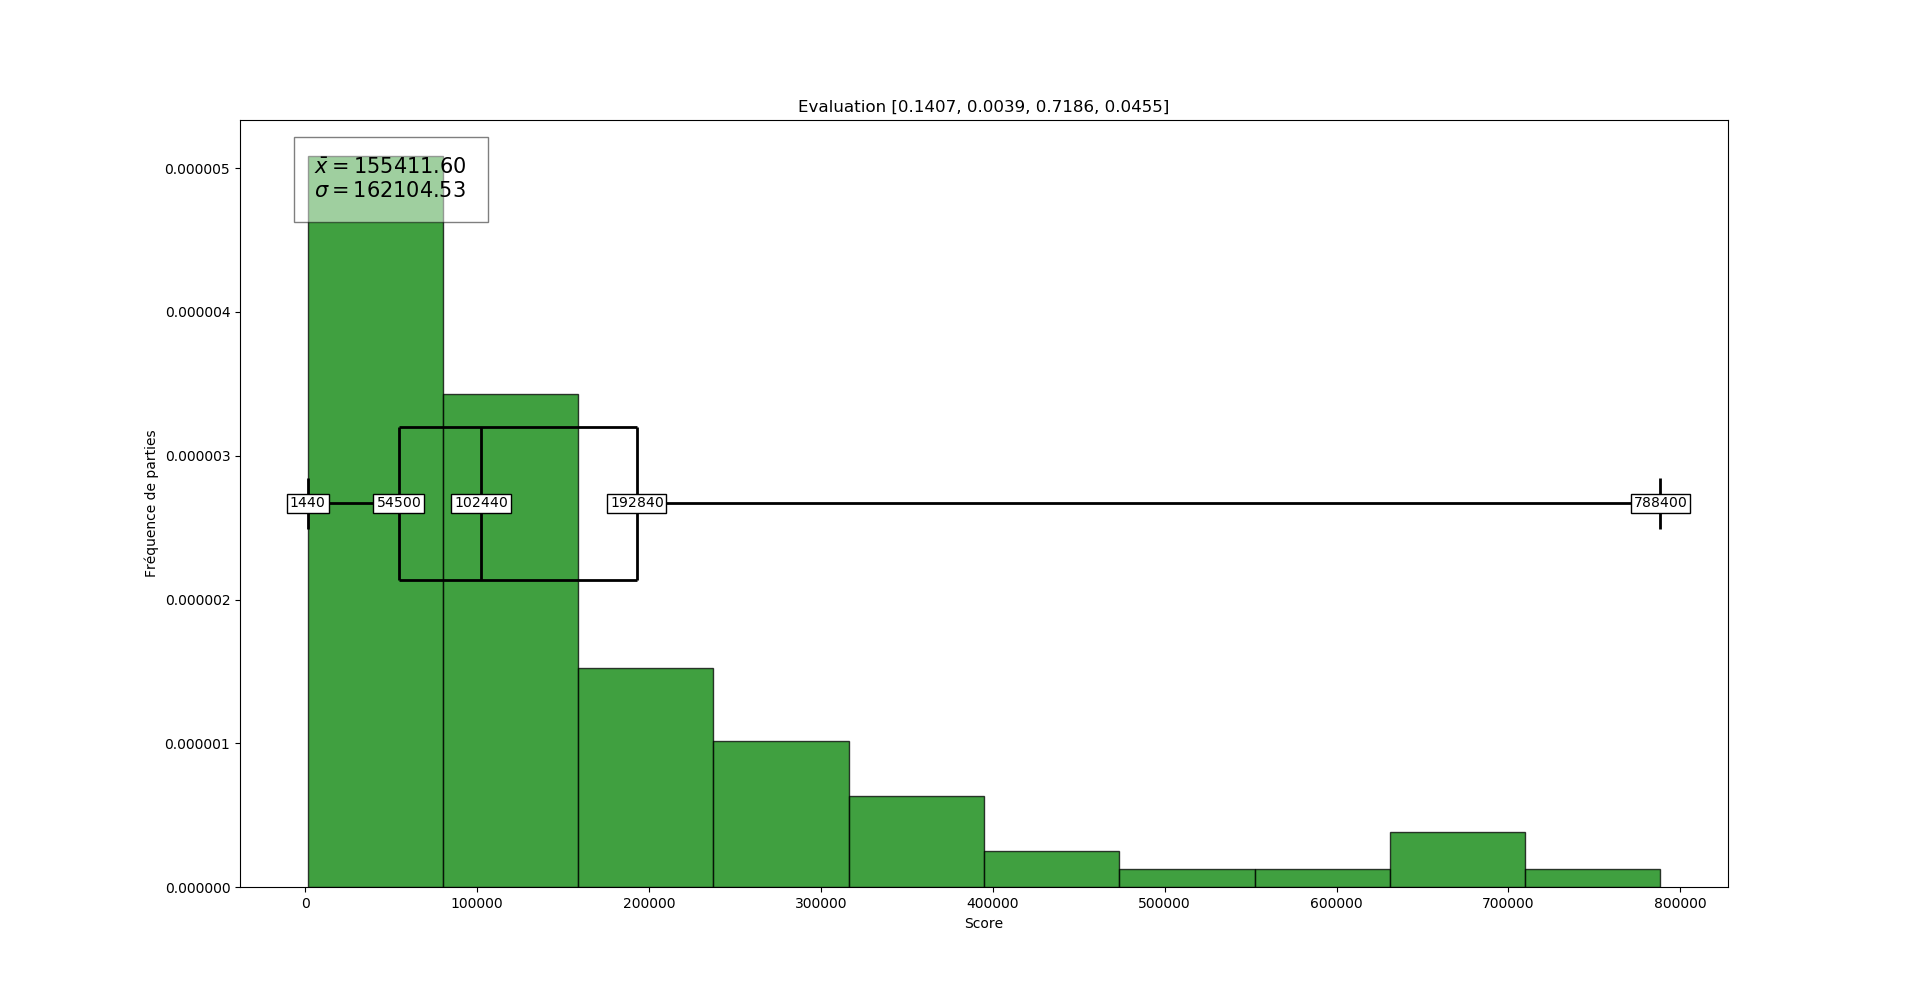
\includegraphics[scale=0.35]{media/results/Stats_Eval_0,1407_0,0039_0,7186_0,0455.png}

\newpage

\subsection{Dernier exemple}

Cette dernière optimisation a tourné pendant 3 semaines et nous avons dû l'interrompre après seulement 9 générations.

 Paramètres :
 
 \begin{itemize}
 	\item \pyth{population\_size : 1000}
 	\item \pyth{nb\_games\_played : 100}
 	\item \pyth{vector\_encoding : float}
 	\item \pyth{parents\_selection\_method : tournament}
 	\item \pyth{old\_generation\_policy : best}
 	\item \pyth{evaluation\_criteria : scores}
 	\item \pyth{proba\_mutation = 0.05}
 	\item \pyth{mutation\_rate = 0.20}
 	\item \pyth{percentage\_for\_tournament = 0.10}
 	\item \pyth{percentage\_new\_offspring = 0.30}
 \end{itemize} 

\medskip

Voici le résultats sur 100 parties :

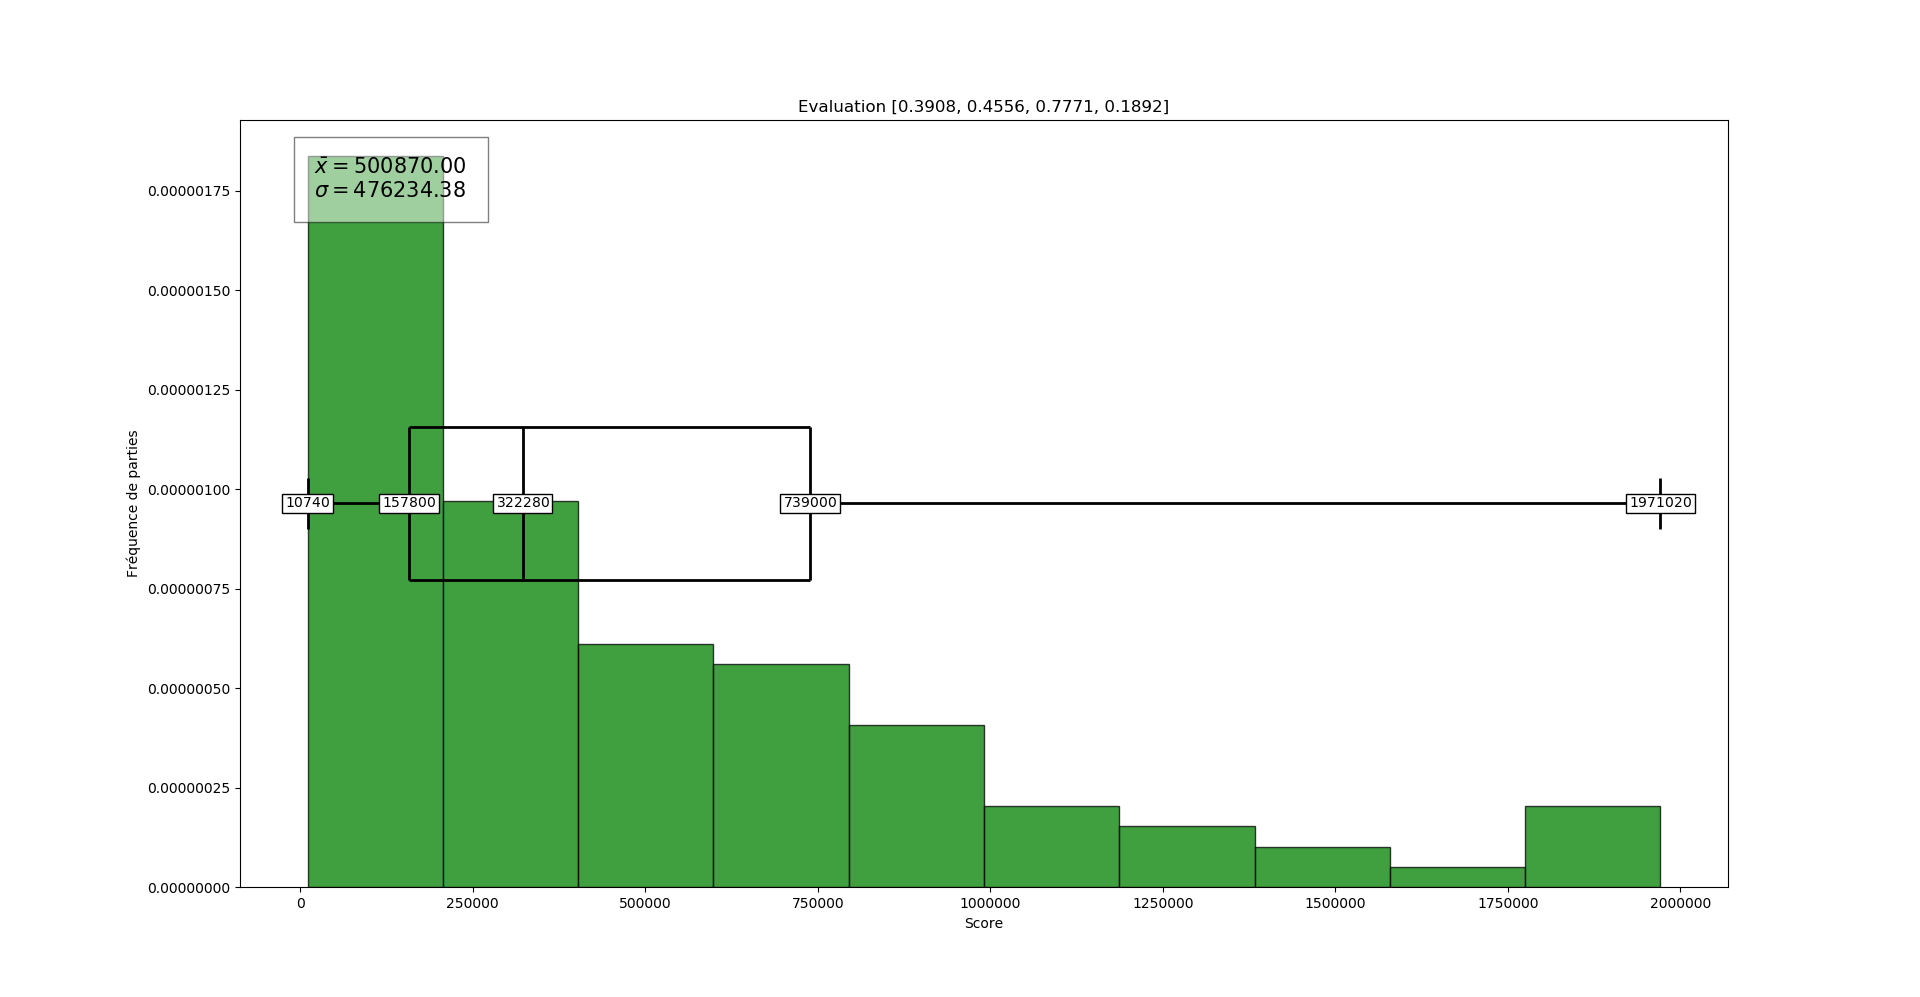
\includegraphics[scale=0.35]{media/results/Stats_Eval_0,3908_0,4556_0,7771_0,1892.png}

\newpage

\section{Optimisation par Q-Learning}

Dans la mesure où on ne joue qu'avec des dominos, sur de petites grilles, il n'est pas possible de comparer avec les optimisations précédentes.

\medskip

Néanmoins, cette optimisation est capable de trouver une stratégie pour jouer sans fin sur une grille de $8\times 8$ en prenant 50000 épisodes d'apprentissage.

